To train and assess our method we used the datasets of protein decoys from the CASP competition \cite{moult2014critical}. 
We took the datasets CASP7 - CASP10 as the training set and the CASP11 dataset as the test set.
We optimized side chain conformation of the training and test sets using SCWRL4 program \cite{krivov2009improved}.
The training and test sets have 564 and 83 targets correspondingly. For each target the training dataset has 
on average 282 decoys. The test dataset is split into two subsets: Stage1 with 20 selected decoys for each target and Stage2 with 150 decoys
for each. The native structures were not included in the datasets nor during the training procedure
neither during the testing phase. 

The distribution of target sequences lengths are shown on Fig. \ref{Fig:dataLengthDist}. We see,
that these two datasets cover the same interval of sequence lengths. However, to ensure that the training 
and test sets are significantly different we aligned all the sequences from the test set agains all the training 
set sequences using blasp tool \cite{altschul1990basic}. The most significant alignments are shown in the Table \ref{Tbl:datasetsSimilarity}.
We see that less than 15\% of the targets in the test set have similar sequence stretches to the targets in the training set.

To assess the evolutionary similarity of the two datasets we found the pfam family of each target in the training and the 
test sets and computed the overlap between the families in both datasets. We used HMMER tool with the e-value cutoff 1.0 to 
find the pfam family of a target \cite{finn2016pfam}. Table \ref{Tbl:SharedPFam} shows the targets in test and train sets, that share a family. We 
estimate that approximately 25\% of test set targets share a family with roughly 10\% of the targets in the training set.

Also, we classified the structures in the training and test sets using ECOD database \cite{cheng2014ecod}. This database provides classification of 
RCSB PDB dataset \cite{berman2000protein} into a tree-like structure with nodes being: architecture type, X-, H-, T- and F-groups. One 
protein chain can have multiple structural domains. 
The higher the branch two protein 
domains occupy, the more they are structuraly similar. Figure \ref{Fig:foldsGraph} shows the classification of the test set into ECOD classes. The 
branches drawn with black are those that have at least one domain structure in the training set, belonging to them. The grey branches are the 
classes unique to the test set. We see that among all the architectural types, spanned by the test set, only four are overlapping completely
between training and test sets. They are: a/b barrels, beta duplicates or obligate multimers, a+b complex topology and a+b four layers.
The targets T0773, T0797, T0816 are excluded due to absent ECOD classification, targets T0820, T0823, T0824, T0827, T0835, T0836 were 
excluded due to absense of their structures in the RCSB database.

The overview of the train and test sets overlap is presented on Fig. \ref{Fig:summaryTable}. 
For each target domain we computed the closest domain in the 
training set and denoted this overlap with black tiles in the A, X, H, T, F rows. The family and clans assignment has gaps with no information, 
denoted with grey tiles. When target in the test set has at least one target in the training set belogning to the same family or clan the black 
tile appears. Finally, if sequences of two targets have alignment with the e-value smaller than $1\cdot10^{-4}$, the tile in the alignment row is 
black.

\begin{figure}[H]
    \centering
    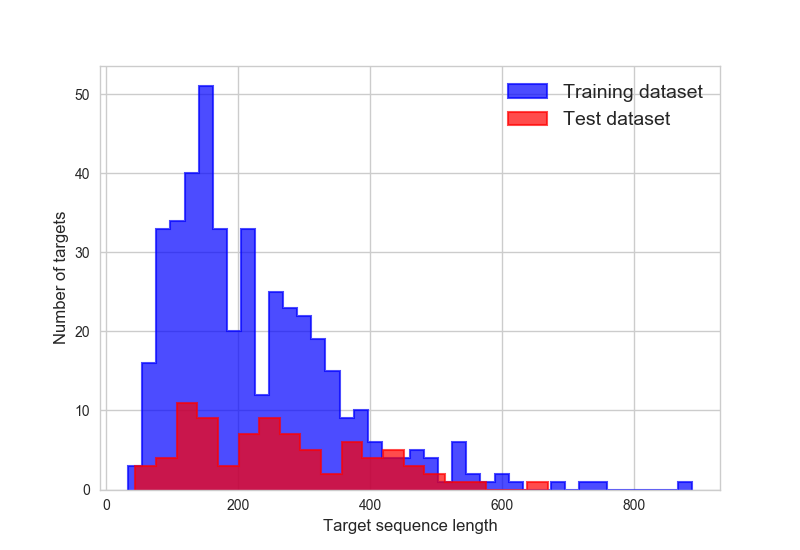
\includegraphics[width=\linewidth]{Fig/datasetLengthDistributions.png}
    \caption{The distributions of sequence lengths for targets in training set(blue) and test set(red).}
    \label{Fig:dataLengthDist}
\end{figure}

\begin{table}[H]
\begin{center}
\begin{tabular}{ c | c | l }
    
    Test set id & Closest training set id & E-value \\
    \hline
    T0768 & T0690 & 2.7e-13\\
    T0770 & T0645 & 1.79e-13\\
    T0772 & T0518 & 1.89-07\\
    T0776 & T0707 & 3.98e-05\\
    T0783 & T0699 & 1.19e-22\\
    T0798 & T0308 & 9.57e-06\\
    T0813 & T0398 & 2.45e-05\\
    T0819 & T0636 & 8.66e-15\\
    T0854 & T0324 & 2.13e-13\\
\end{tabular}
    
    \caption {The closest homologs from training and test sets. The search was performed using blastp tool. The database was constructed from 
    the training set sequences; test sequences were queried against this database. We used 1e-4 e-value cutoff to filter only significant 
    alignments.}
    \label{Tbl:datasetsSimilarity}
\end{center}
\end{table}


\begin{table}[H]
\begin{center}
\begin{tabular}{ l | l | l }

    Common family & Test set target & Train set targets \\
    \hline
    PF00795.21 & T0794 & T0542 \\ \hline
    PF13472.5 & T0776 & T0448, T0297, T0286, T0750 \\ \hline
    PF03807.16 & T0813 & T0398, T0393, T0702 \\ \hline
    PF00266.18 & T0801 & T0339, T0697 \\ \hline
    PF01128.18 & T0783 & T0699, T0420 \\ \hline
    PF07949.11 & T0780 & T0572 \\ \hline
    PF13577.5 & T0815 & T0752, T0736 \\ \hline
    PF12804.6 & T0783 & T0593, T0699, T0420 \\ \hline
    PF13242.5 & T0854 & T0371, T0341, T0303, T0324, T0330, T0329, T0418 \\ \hline
    PF13306.5 & T0768 & T0690, T0671, T0713, T0653 \\ \hline
    PF12741.6 & T0770 & T0664, T0645, T0532 \\ \hline
    PF00025.20 & T0798 & T0308 \\ \hline
    PF12872.6 & T0792 & T0549 \\ \hline
    PF03446.14 & T0813, T0851 & T0398, T0393, T0702 \\ \hline
    PF00155.20 & T0801, T0819 & T0591, T0636, T0436, T0697 \\ \hline
    PF13419.5 & T0854 & T0371, T0341, T0303, T0379, T0324, T0330, T0329, T0418, T0635 \\ \hline
    PF12680.6 & T0815 & T0451, T0475 \\ \hline
    PF06439.10 & T0772 & T0518 \\ \hline
    PF12771.6 & T0770 & T0664, T0645, T0532 \\ \hline
    PF08477.12 & T0798 & T0308 \\ \hline
    PF00657.21 & T0776 & T0297, T0286, T0679 \\ \hline
    PF00071.21 & T0798 & T0308 \\ \hline
    PF00702.25 & T0854 & T0303, T0324, T0330, T0329, T0418, T0635 \\ \hline
    PF01926.22 & T0798 & T0308 \\ \hline
    PF12697.6 & T0764 & T0672 \\ \hline
\end{tabular}
    
\caption {Targets from test and train sets that belong to the same PFam family \cite{}. To obtain the family of a target we used HMMER search \cite{}.
Out of 564 targets in training and 83 targets in test sets 403 and 65 targets correspondingly had the families assigned to them. In total, this 
table contains 25 families, that correspond to the distinct 25 PFam clans. Alltogether, this table contains 16 test targets and 42 training targets.}
\label{Tbl:SharedPFam}
\end{center}
\end{table}

\begin{figure}[H]
    \centering
    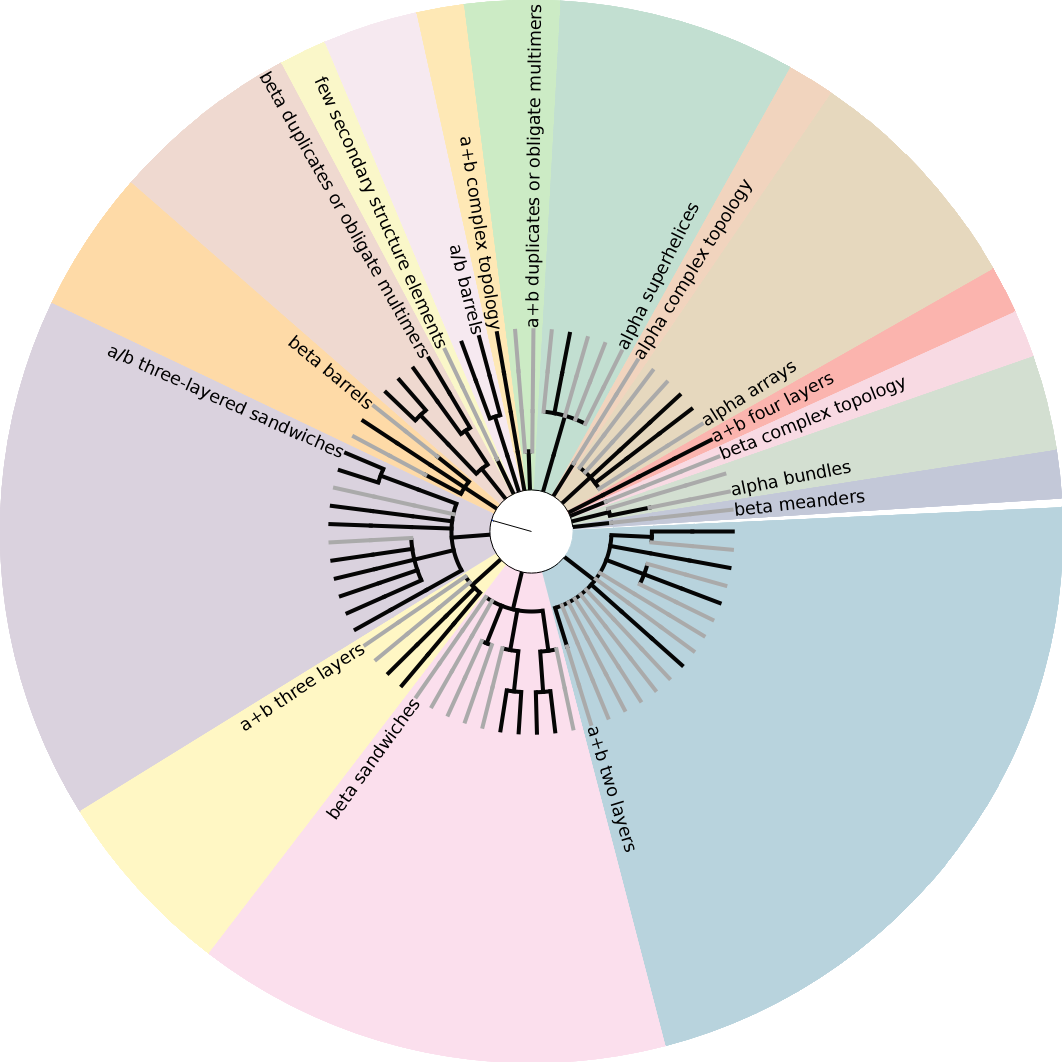
\includegraphics[width=\linewidth]{Fig/folds_graph.png}
    \caption{The classification of the test set into ECOD structural classes (architecture type, X-, H-, T- and F- groups). The architecture 
    types are shown in the outer circle of the diagram. The grey lines denote test set classes that have no respective representative in the 
    training set. The black lines show the classes that have representatives in both training and test sets. We do not show the F-groups, because
    they have litle overlap among the training and test sets.}
    \label{Fig:foldsGraph}
\end{figure}

\begin{figure}[H]
    \makebox[\textwidth]{
    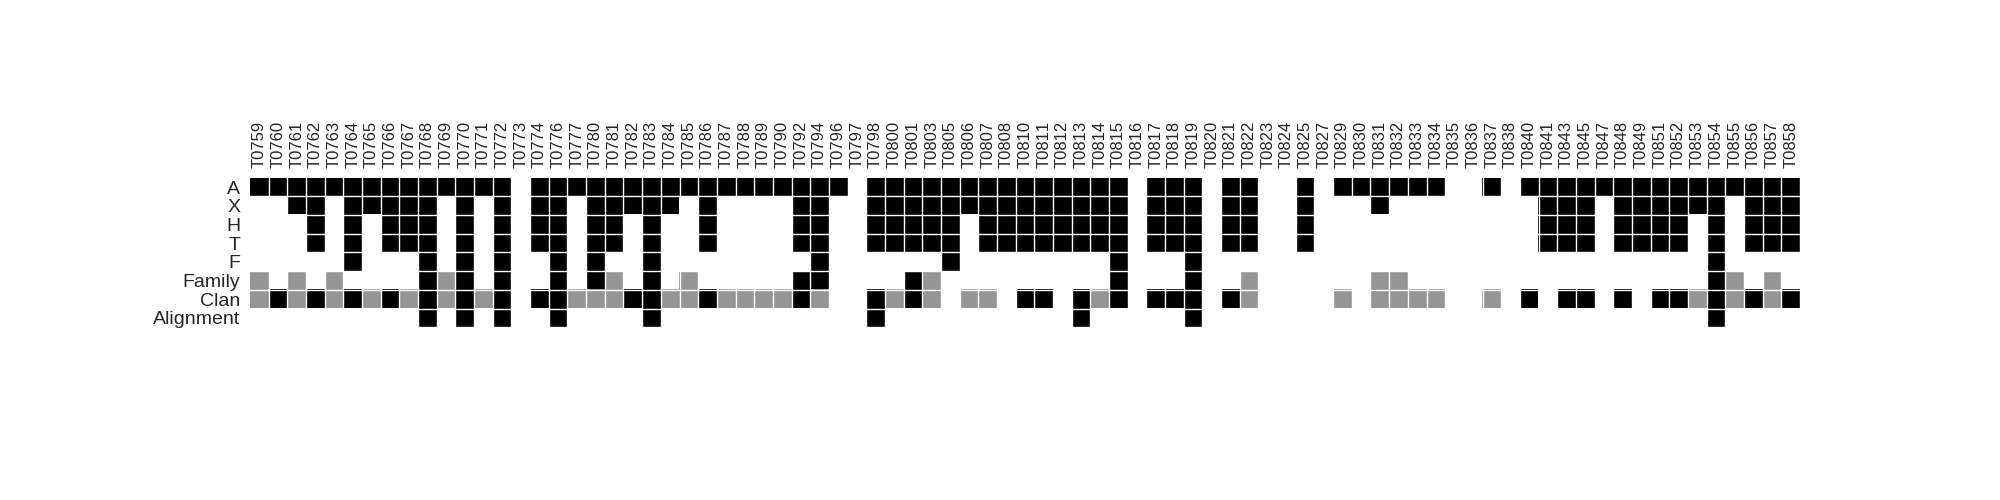
\includegraphics[width=\paperwidth]{Fig/summary_table.png}
    }
    \caption{The overview of the overlap between training and test datasets. The first 5 rows correspond to the ECOD classification of 
    domains (A is the architecture type and X, H, T and F are the classes). The structure in the dataset has
    a domain that belongs to the same group as a domain from the training set with the matching class if the corresponding tile colored black.
    The closest match for each target is shown. The family and class rows show if the target was not assigned to any family of clan (grey) or 
    if there is a target in the training set with the same family or clan (black). The alignment row shows the targets that have an alignment
    with a target in the training set with e-value less than $1\cdot10^{-4}$.}
    \label{Fig:summaryTable}
\end{figure}